% vim:encoding=utf8 ft=tex sts=2 sw=2 et:

\documentclass{classrep}
\usepackage[utf8]{inputenc}
\usepackage{color}
\usepackage{graphicx}

\studycycle{Informatyka, studia dzienne, mgr II st.}
\coursesemester{I}

%\coursename{Angelologia teoretyczna i stosowana}
\coursename{Obliczenia inteligentne}
\courseyear{2010/2011}

\courseteacher{Michał Pryczek}
\coursegroup{Środa, 14:30}

\author{
  \studentinfo{Leszek Wach}{169513} \and
  \studentinfo{Michał Janiszewski}{169485} \and
}

\title{Zadanie: Analiza danych biomedycznych}
\svnurl{https://serce.ics.p.lodz.pl/svn/labs/oi/mpat_sr1430/wacjan/OI-MP/@182}

\begin{document}
\maketitle

\section{Cel}
Zadanie polegało na analizie danych biomedycznych uzyskanych dzięki technice płytek genowych(mikromacierzy). Zadanie składało się z dwóch etapów: redukcji ilości cech opisujących osobnika oraz stworzenia klasyfikatora który byłby w stanie określić na podstawie zredukowanego zbioru cech przynależność osobnika do jednej z klas. W naszym przypadku druga część zadania polegała na stworzeniu klasyfikatora potrafiącego rozpoznać, który typ napoju zawierających kwasy tłuszczowe wypiła badana osoba. W doświadczeniu wykorzystano dwa typy napojów: PUFA i SUFA.

\section{Wprowadzenie}
\subsection{Micromacierze}
Technika mikromacierzy pozwala na jednoczesną analizę ekspresji tysięcy genów. W celu stworzenia mikromacierzy pobierane są dwie grupy komórek: testowa i odniesienia.
Z pobranych komórek zostają wyodrębnione łańcuch mRNA. Ponieważ mRNA łatwo ulega degradacji poddaje się je procesowi odwrotnej transkrypcji, otrzymując komplementarne cDNA.\\ \indent Następnie cDNA zostaje zaznaczone barwnikiem różnym dla komórek testowych i odniesienia. Barwnik pozwala zidentyfikować obecność cząsteczki na płytce. Jako barwnika najczęściej używa się farb fluorescencyjnych.\\
\indent Kolejnym etapem jest hybrydyzacja polegająca an zanurzeniu płytki w roztworze zabarwionego cDNA. Cząsteczki cDNA łączą się z punktami(sondami) na płytce zawierającymi komplementarne sekwencje DNA.\\
\indent Po zakończeniu hybrydyzacji płytka zostaje umieszcona w skanerze gdzie następuje odczyt ekspresji genów czyli zabarwienia punktów płytki \footnote{\cite{metodyklasyfikacji}}.
\subsection{Metoda k-średnich}
W zadaniu użyto metody k-średnich. Jest to jedna z metod grupujących pozwalająca znaleźć grupy genów o zbliżonej ekspresji. Metoda polega na utworzeniu pewnej liczby grup i przypisania elementów do grup bazując na pewnej mierze podobieństwa. Obiekty podobne do siebie powinny być umieszczane w tej samej grupie. Metoda dąży do minimalizacji różnic wewnątrz grup i maksymalizacji różnic między różnymi grupami\footnote{\cite{metodyklasyfikacji}}\\\\
\textbf{Opis algorytmu}
\begin{enumerate}

\item Wyznaczenie k punktów wyznaczających początkowe centroidy grup.

\item Przypisanie każdego obiektu do grupy, dla której odległość między jej centroidem a danym obiektem jest najmniejsza według określonej miary.

\item Wyliczenie nowych centroidów w powstałych grupach np. jako średnią arytmetyczną obiektów w grupie.

\item Powtarzanie kroków 2 i 3 aż do zadanej liczby iteracji lub do momentu, gdy w trakcie iteracji żaden z obiektów nie zmieni grupy.\\
\end{enumerate}
Metoda k-średnich wymaga znania z góry liczby grup, na które zostanie podzielony zbiór. Wyznaczenie początkowych centroidów może odbyć się losowo i tak też było w naszym programie.
\subsection{Miary podobieństwa}
W metodzie k-średnich do wyznaczania wartości podobieństwa dwóch wektorów używamy poniższych miar.\\

Odległość euklidesowa:
\begin{equation}
  e(x, y) = \sqrt{\displaystyle \sum_{i = 1}^{N} (x_i - y_i)^2}
\end{equation}

Współczynnik korelacji Pearsona:
\begin{equation}
  p(x,y) = \frac{\displaystyle\sum_{i = 1}^{N}(x_i - \bar{x})(y_i -
\bar{y})}{\sqrt{\displaystyle \sum_{i=1}^N (x_i - \bar{x})^2}\sqrt{\displaystyle
\sum_{i=1}^N (y_i - \bar{y})^2}}
\end{equation}

Współczynnik korelacji Spearmana:
\begin{equation}
  p(x,y) = \frac{\displaystyle\sum_{i = 1}^{N}(x_i - \bar{x})(y_i -
\bar{y})}{\sqrt{\displaystyle \sum_{i=1}^N (x_i - \bar{x})^2 \displaystyle
\sum_{i=1}^N (y_i - \bar{y})^2}}
\end{equation}

gdzie $\bar{x}$  to wartość średnia wektora $x$, a $\bar{y}$ wartość średnia wektora $y$.

\subsection{Wielowarstwowy Perceptron}	
Perceptron jest przykładem jednokierunkowej sieci, w której neurony są ułożone w warstwy.
Każda warstwa składa się z pewnej określonej liczby neuronów. Pierwsza warstwa składa się z neuronów kopiujących czyli wyjście każdego neuronu jest takie samo jak jego wejście. Warstwę pierwszą określa się jako warstwę wejściową. Liczba neuronów w warstwie wejściowej	
określa liczbę wejść sieci. Następnie w sieci znajduje się szereg warstw	
ukrytych. Ostatnia warstwa jest warstwą wyjściową. Ilość neuronów w	
warstwie wyjściowej określa liczbę wyjść sieci. Sieć jest tak zorganizowana, że	
wyjście każdego neuronu w warstwie $k$ jest połączone ze wszystkimi neuronami w
warstwie $k+1$ (z wyjątkiem warstwy wyjściowej).			
\subsection{Nauka sieci}
Algorytm wstecznej propagacji błędu jest wykorzystywany w celu minimalizacji błędu sieci.
Jest to metoda określana jako nauka z nauczycielem. Nauka z nauczycielem polega na przekazywaniu do sieci pewnych wartości i porównywaniu wyników sieci z pewnymi wartościami oczekiwanymi. W trakcie tego typu nauki obliczany jest błąd wyniki i wagi neuronów sieci są modyfikowany w taki sposób aby w następnej iteracji błąd był mniejszy.

W przypadku sieci wielowarstwowych mamy informacje tylko o błędzie popełnionym przez ostatnią, wyjściową warstwę.	
W takiej sytuacji stosuje się algorytm wstecznej propagacji błędu. Polega on na	
tym, że najpierw wyznaczamy wartości błędu dla wszystkich neuronów z	
ostatniej warstwy o numerze $K$:	
\begin{equation}	
  \delta_i^K = y_i - r_i	
\end{equation}	
gdzie $i$ jest numerem neuronu ($i = 1, 2, ...,N_K - 1$, $N_K$ \ppauza liczba	
neuronów w $K$-tej warstwie), $y_i$ \ppauza wartość oczekiwana na $i$-tym	
neuronie, $r_i$ \ppauza wartość otrzymana na danym neuronie.		
Następnie obliczamy wartości błędów dla neuronów w pozostałych warstwach sieci:	
\begin{equation}	
  \delta_i^{K-1} = \displaystyle \sum_{j=1}^{N_{K}} w_i^{jK} \delta_j^K	
\end{equation}	
gdzie $w_i^{jK}$ oznacza $i$-ty element wektora wag neuronu o numerze $j$ z	
$K$-tej warstwy ($i=1,2,...,N_{K-1}$, $N_{K-1}$ jest liczbą neuronó w	
$K-1$-szej warstwie).		
Aby zwiększyć zbieżność algorytmu stosuje się współczynnik momentum $\alpha$:
\begin{equation}	
\Delta w_i^{jK(k)} = \eta \delta_i^{K-1} u_i^K + \alpha \Delta w_i^{jK(k-1)}	
\end{equation}	
gdzie: $\Delta w_i^{jK(k)}$ \ppauza zmiana wagi $i$ w $j$-tym neuronie w	
$K$-tej warstwie w $k$-tej iteracji, $u_i^K$ \ppauza $i$-ta wartość wejściowa
dla $K$-tej warstwy, $\eta$ \ppauza współczynnik uczenia, $\alpha$ \ppauza	
współczynnik momentum. Obliczoną wartość zmiany wag dodajemy do aktualnych	
wag poszczególnych neuronów.

\section{Opis implementacji}
W ramach zadania powstała aplikacja napisana w języku C++ z wykorzystaniem biblioteki Qt. Program wczytuje dane z pliku tekstowego i przechowuje je w obiekcie klasy \verb+MicroArray+. Do prawidłowego wczytania danych wymagane jest ustalenie liczby grup oraz ich liczebności w pliku z danymi.

Po wczytaniu danych zostaje uruchomiona metoda \verb+run()+ na rzecz obiektu klasy \verb+Kmeans+. Metoda ta implementuje algorytm k-średnich. Do prawidłowego działania metody wymagane jest ustalenie liczby grup oraz maksymalnej liczby iteracji. Wynikiem metody są liczebności grup oraz lista ostatecznych centroidów należących do tych grup. Na podstawie centroidów program wybiera przedstawicieli poszczególnych grób. Przedstawiciele grup tworzą dane treningowe wykorzystywane w procesie nauki sieci.

Za naukę i testowanie sieci odpowiada klasa \verb+Utils+. W programie wykorzystano bibliotekę FANN 2.1.0 zawierającą implementację perceptronu.

\section{Materiały i metody}
Badania zostały wykonane na zestawie oznaczonym indeksem GSE13466\footnote{\cite{research}}. Zestaw zawiera profile genów pobranych z komórek krwi obwodowej od 21 młodych mężczyzn. \\W zestawie można wyróżnić cztery klasy.
\begin{itemize}
\item[•] 6 godzin przed spożyciem PUFA(wielonienasycone kwasy tłuszczowe)
\item[•] 6 godzin po spożyciu PUFA
\item[•] 6 godzin przed spożyciem SFA(nasycone kwasy tłuszczowe)
\item[•] 6 godzin po spożyciu SFA\\
\end{itemize}

Metodę k-średnich przetestowano dla wartości k równego: 100, 200 oraz 400. We wszystkich przypadkach liczba iteracji wynosiła 100. Wyniki grupowania można zobaczyć na rysunkach do \ref{euclidean.100} do \ref{spearman.400}.

Po przetestowaniu metody k-średnich przeprowadzono 4 testy obejmujące stworzenie klasyfikatora. Algorytm k-średnich był za każdym razem wykonywany oddzielnie dla grupy SUFA i grupy PUFA. W każdym z testów uczono sieci z momentum równym 0.6 i współczynnikiem nauki równym 0.6. Jako algorytm nauki wykorzystano dostarczony z biblioteką FANN algorytm FANN\_RPROP. Funkcje aktywacji warstwy ukrytej i wyjściowej ustawiono na FANN\_SIGMOID\_SYMETRIC.

W trakcie analizy wyników za poprawny wynik klasyfikatora(sieci) uznawano wartości różniące się od wartości oczekiwanej nie więcej niż o 0.01.\\\\
\textbf{Ogólny przebieg testów:}
\begin{itemize}
\item[•] uruchomienie algorytmu k-średnich,
\item[•] wybranie przedstawicieli wygenerowanych grup,
\item[•] zapisanie danych w formacie umożliwiającym naukę sieci, czyli to co wcześniej było kolumnami macierz teraz jest wektorami wejściowymi sieci, określenie oczekiwanych wyjść sieci(1 dla PUFA, -1 dla SUFA),
\item[•] podzielenie zbioru danych treningowych na cztery rozłączne zbiory,
\item[•] uruchomienie nauki czterech sieci neuronowych z których każda ma inny zbiór walidujący(jeden z czterech wyznaczonych w poprzednim kroku), wszystkie sieci razem stanowią klasyfikator,
\item[•] policzenie średniego błędu dla wszystkich sieci, jest to średni błąd stworzonego klasyfikatora,
\item[•] przetestowanie klasyfikatora na całym zbiorze danych.\\
\end{itemize}
\textbf{Test1}\\
liczba grup = 50\\
liczba iteracji algorytmu k-średnich = 100\\
liczba sieci = 4\\
liczba neuronów warstwy ukrytej = 10\\
Wektor wejściowy przekazywany do sieci neuronowej składał się z wartości genów zarówno przed jak i po spożyciu kwasów tłuszczowych.\\\\
\textbf{Test2}\\
liczba grup = 400\\
liczba iteracji algorytmu k-średnich = 100\\
liczba sieci = 4\\
liczba neuronów warstwy ukrytej = 30\\
Wektor wejściowy przekazywany do sieci neuronowej składał się z wartości genów zarówno przed jak i po spożyciu kwasów tłuszczowych.\\\\
\textbf{Test3}\\
liczba grup = 400\\
liczba iteracji algorytmu k-średnich = 100\\
liczba sieci = 4\\
liczba neuronów warstwy ukrytej = 20\\
Wektor wejściowy przekazywany do sieci neuronowej składał się tylko z wartości genów po spożyciu kwasów tłuszczowych.\\\\
\textbf{Test4}\\
liczba grup = 600\\
liczba iteracji algorytmu k-średnich = 100\\
liczba sieci = 4\\
liczba neuronów warstwy ukrytej = 35\\
Wektor wejściowy przekazywany do sieci neuronowej składał się z wartości genów zarówno przed jak i po spożyciu kwasów tłuszczowych.\\\\
Wyniki wszystkich testów przedstawiono w tabeli \ref{testTab1}.

\section{Wyniki}
Na rysunkach od \ref{euclidean.100} do \ref{spearman.400} przedstawiono wyniki działania algorytmu k-średnich. W tabeli \ref{testTab1} zamieszczono wyniki testów klasyfikatorów uzyskanych w trakcie realizacji zadania.
\begin{figure}
  \centering
  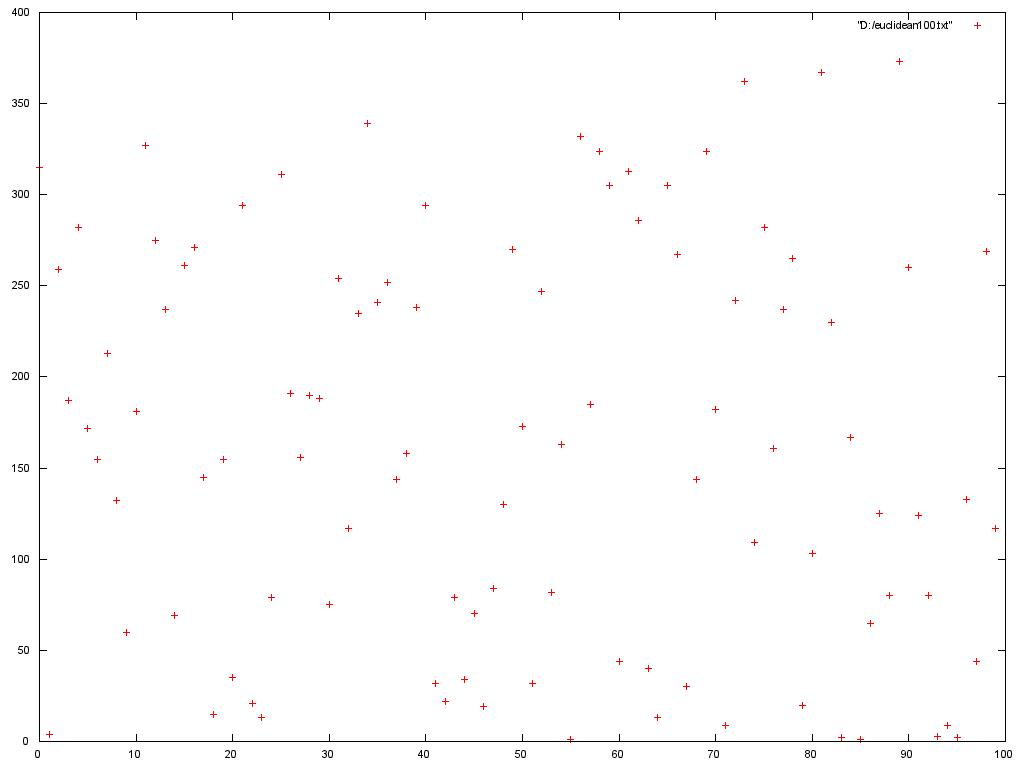
\includegraphics[width=10cm]{img/euclidean100.png}
  \caption{Wykres przedstawiający liczbę cech przyporządkowanych poszczególnym
grupom dla $k=100$, Odległość Euklidesa}
  \label{euclidean.100}
\end{figure}

\begin{figure}
  \centering
  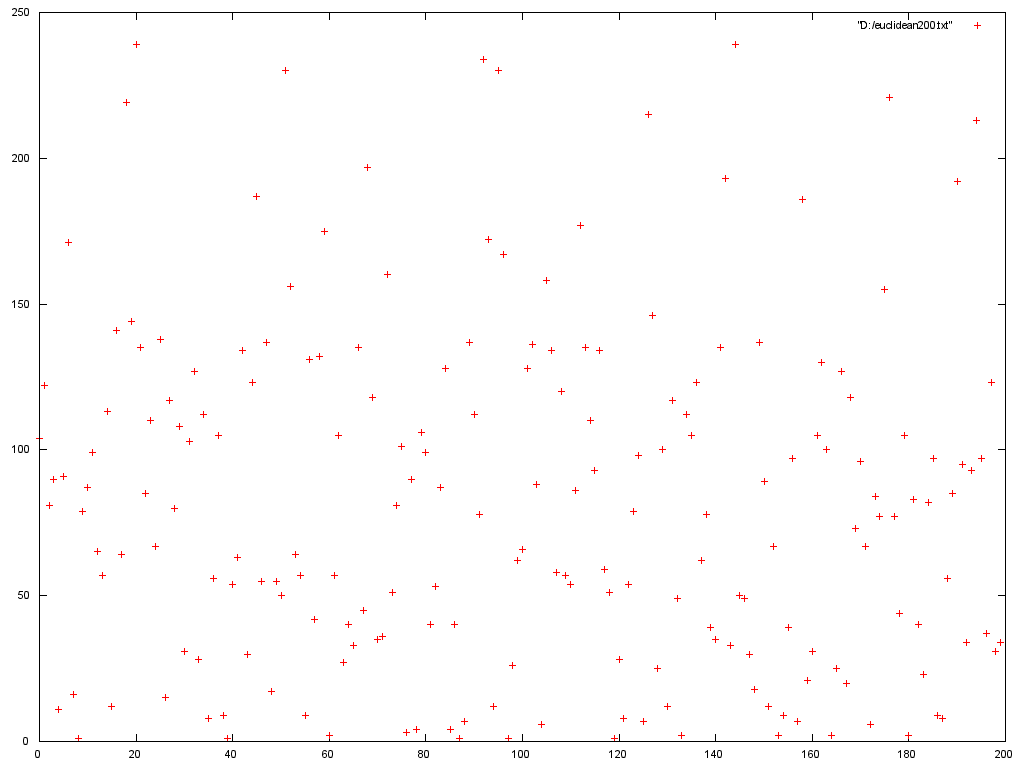
\includegraphics[width=10cm]{img/euclidean200.png}
  \caption{Wykres przedstawiający liczbę cech przyporządkowanych poszczególnym
grupom dla $k=200$, Odległość Euklidesa}
  \label{euclidean.200}
\end{figure}


\begin{figure}
  \centering
  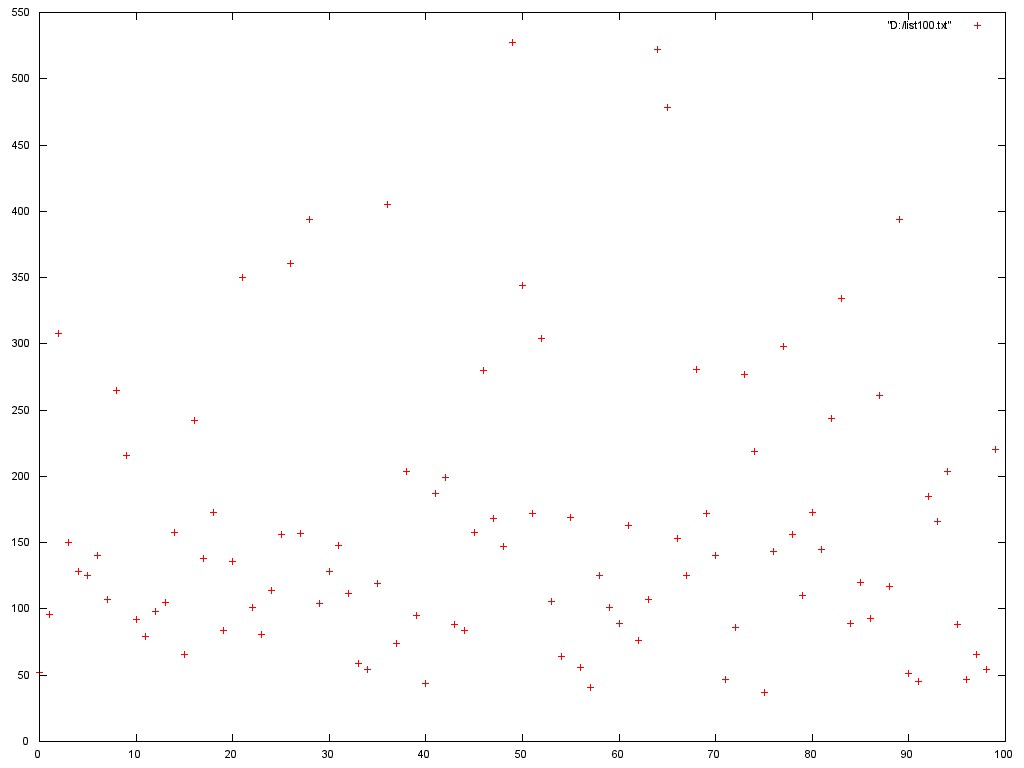
\includegraphics[width=10cm]{img/pearson100.png}
  \caption{Wykres przedstawiający liczbę cech przyporządkowanych poszczególnym
grupom dla $k=100$, Współczynnik korelacji Pearsona}
  \label{pearson.100}
\end{figure}

\begin{figure}
  \centering
  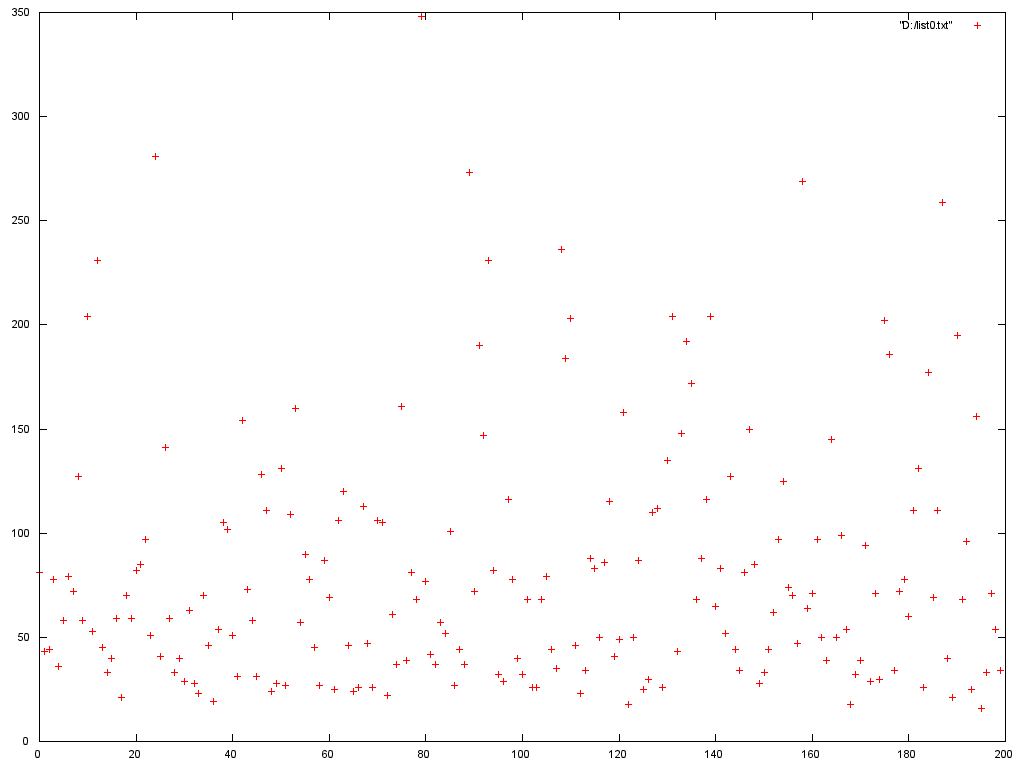
\includegraphics[width=10cm]{img/pearson200.png}
  \caption{Wykres przedstawiający liczbę cech przyporządkowanych poszczególnym
grupom dla $k=200$, Współczynnik korelacji Pearsona}
  \label{pearson.200}
\end{figure}

\begin{figure}
  \centering
  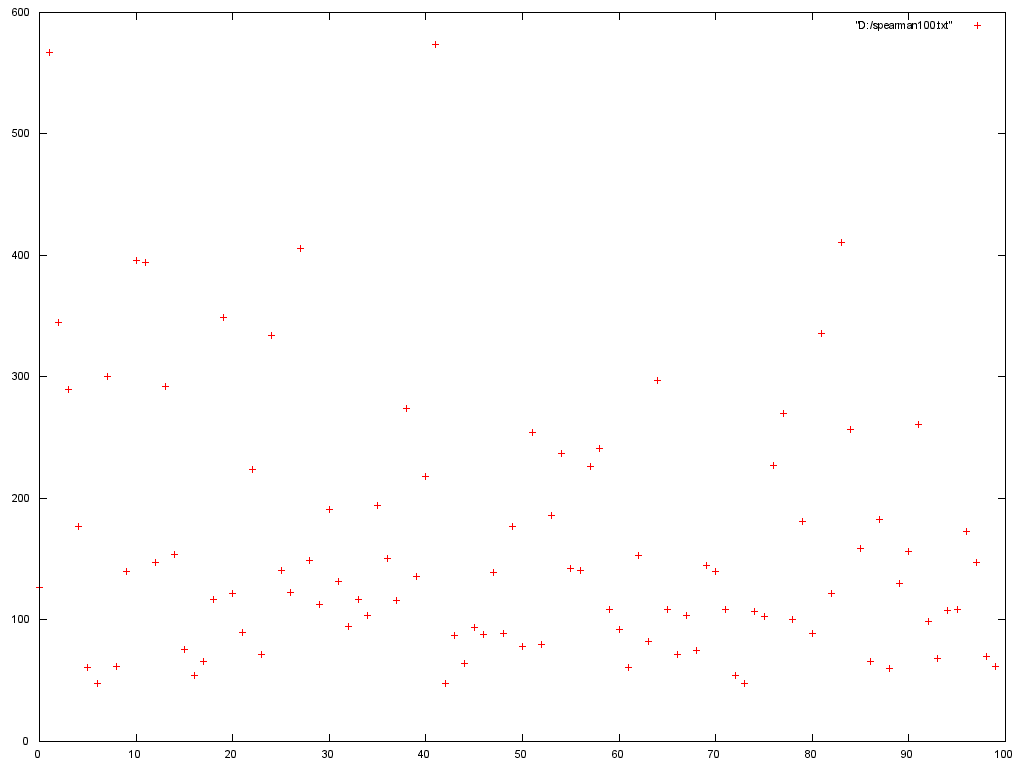
\includegraphics[width=10cm]{img/spearman100.png}
  \caption{Wykres przedstawiający liczbę cech przyporządkowanych poszczególnym
grupom dla $k=100$, Współczynnik korelacji Spearmana}
  \label{spearman.100}
\end{figure}

\begin{figure}
  \centering
  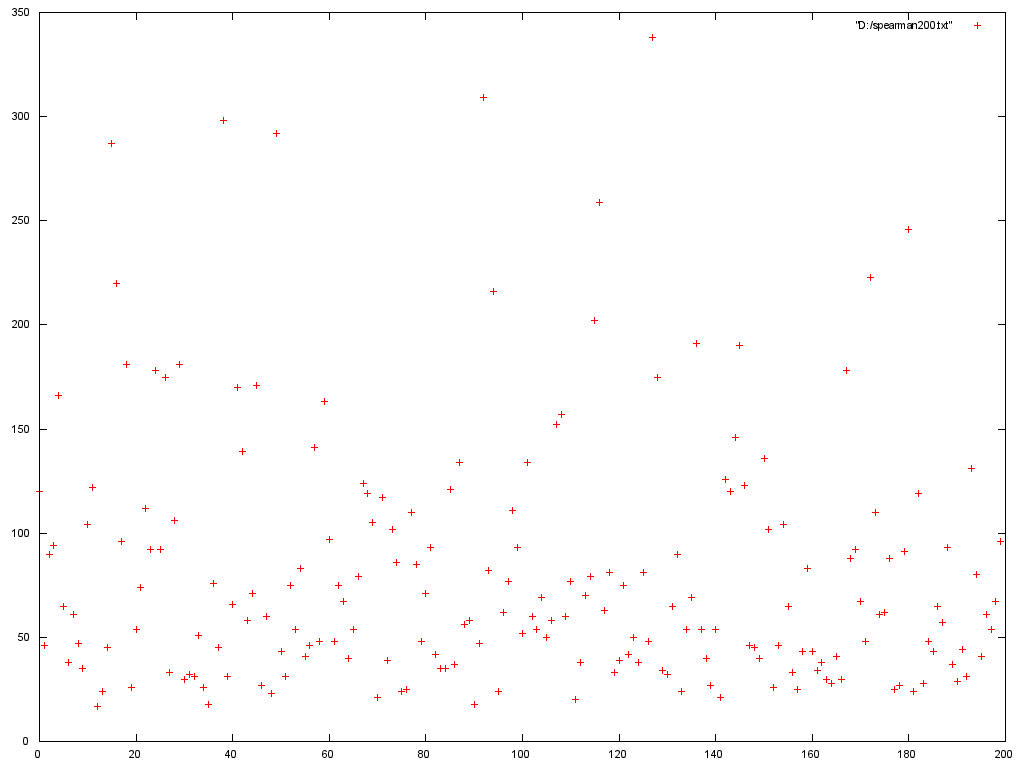
\includegraphics[width=10cm]{img/spearman200.png}
  \caption{Wykres przedstawiający liczbę cech przyporządkowanych poszczególnym
grupom dla $k=200$, Współczynnik korelacji Spearmana}
  \label{spearman.200}
\end{figure}

\begin{figure}
  \centering
  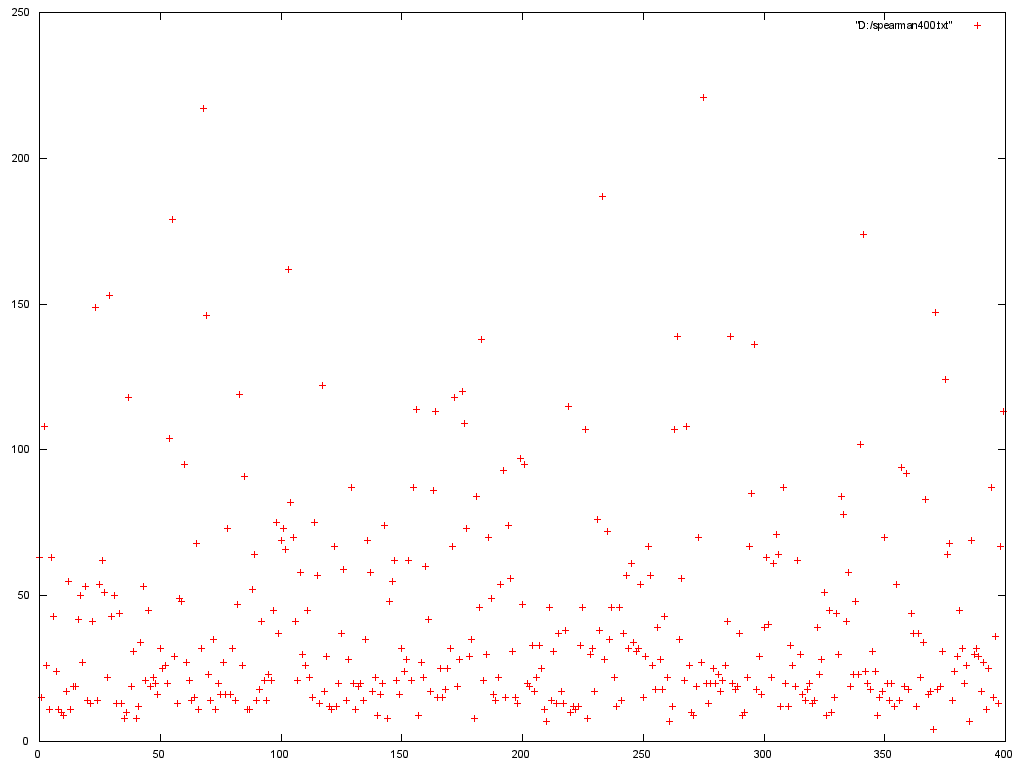
\includegraphics[width=10cm]{img/spearman400.png}
  \caption{Wykres przedstawiający liczbę cech przyporządkowanych poszczególnym
grupom dla $k=400$, Współczynnik korelacji Spearmana}
  \label{spearman.400}
\end{figure}

\begin{table}
\caption{Wyniki testów programu}
\label{testTab1}
\begin{tabular}{|p{1.5cm}|p{2.5cm}|p{2.5cm}|p{2.5cm}|p{2.5cm}|}
 \textbf{Numer testu} & \textbf{Średni błąd klasyfikatora} & \textbf{Procent poprawnie sklasyfikowanych próbek} & \textbf{Procent poprawnie sklasyfikowanych PUFA} & \textbf{Procent poprawnie sklasyfikowanych SUFA} \\ \hline
 1 & 6.011e-05 & 64.00  & 100.00 & 28.57	\\ \hline
 2 & 7.660e-15 & 100.00 & 100.00 & 100.00	\\ \hline
 3 & 1.607e-14 & 100.00 & 100.00 & 100.00 	\\ \hline
 4 & 4.936e-14 & 100.00 & 100.00 & 100.00 	\\ \hline
\end{tabular}
\end{table}

\section{Dyskusja}
Porównując wyniki działania metody k-średnich można zauważyć, że dla współczynników Pearsona i Spearmana liczebności poszczególnych grup są bardziej wyrównane niż dla odległości Euclidesa. W przypadku odległości Euclidesa występuje więcej grup z wieloma elementami, jak i grup, które mają zaledwie kilka elementów.

We wszystkich przeprowadzonych testach uzyskano klasyfikatory dające bardzo dobre rezultaty. Większość próbek została sklasyfikowana poprawnie. W przypadku pierwszego testu liczba grup będąca wynikiem algorytmu k-średnich okazała się zbyt mała aby poprawnie sklasyfikować wszystkie próbki. W pierwszym teście błąd klasyfikatora jest największy.

W kolejnych trzech testach uzyskaliśmy wyłącznie poprawne rezultaty, przy czym wyniki zwracane przez sieci w teście trzecim miały wartości ok. 0.99 lub -0.99 natomiast w testach 2 i 4 zwracane wartości były równe 1.0 lub -1.0. Oznacza to że minimalnie lepsze rezultaty można uzyskać przy pomocy sieci neuronowych uczonych wektorami składającymi się zarówno z wartości genów przed spożyciem jak i po spożyciu kwasów tłuszczowych.

\begin{thebibliography}{0}
\bibitem{metodyklasyfikacji}
\textit{Metody klasyfikacji we wspomaganiu diagnostyki nowotworów techniką płytek genowych}, [online]. [dostęp: 12 maja
2011]. Dostępny w Internecie: http://microarray.republika.pl/index.html
\bibitem{research}
\textit{Series GSE13466}, [online]. [dostęp: 12 maja 2011].
Dostępny w Internecie: http://www.ncbi.nlm.nih.gov/geo/query/acc.cgi?acc=GSE13466
\end{thebibliography}
\end{document}
